\documentclass[a4paper,11pt,authoryear]{elsarticle}
\usepackage[utf8]{inputenc}
\usepackage{amsmath}
\usepackage{tikz}
\usetikzlibrary{positioning}
\usetikzlibrary{calc}
\usetikzlibrary{arrows}
\usetikzlibrary{decorations.pathmorphing,decorations.markings}
\usetikzlibrary{shapes}
\usetikzlibrary{patterns}
\tikzset{
  pics/dist_arc/.style args={#1,#2,#3,#4}{
     code={
       \draw[thick, #4] (-0.25,0.25) -- (0.25,0.25);
       \draw[thick, #4] (-0.5,0) -- (-0.15,0.25);
       \draw[thick, #4] (0.5,0) -- (0.15,0.25);
       \draw[->, thick, #4] (0,0.5) -- (0,0.25);
       \node[#3] (#1) at (0,0) {#2};
     }
  },
  minimum size=2.5em
}

\begin{document}

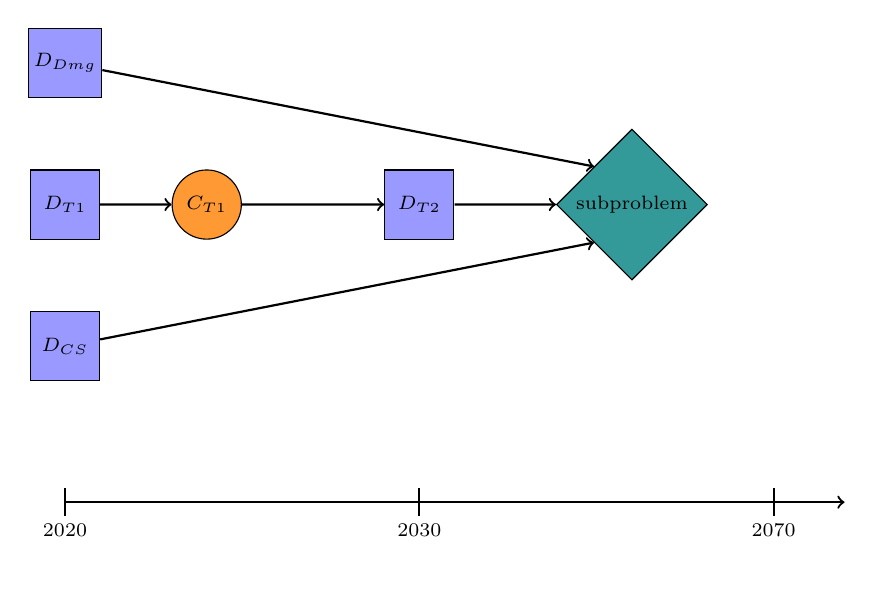
\begin{tikzpicture}
    [decision/.style={fill=blue!40, draw, minimum size=2.5em, inner sep=2pt}, 
    chance/.style={circle, fill=orange!80, draw, minimum size=2.5em, inner sep=2pt},
    value/.style={diamond, fill=teal!80, draw, minimum size=2.5em, inner sep=2pt},
    optimization/.style={ellipse, fill=teal!80, draw, minimum size=2em, inner sep=2pt},
    scale=1.8, font=\scriptsize]
     \node[decision] (D1) at (0, 2)   {$D_{Dmg}$};
     \node[decision] (D2) at (0, 1)   {$D_{T1}$};
     \node[decision] (D3) at (0, 0)   {$D_{CS}$};
     \node[decision] (D5) at (2.5, 1)   {$D_{T2}$};
     \node[chance]   (C2) at (1, 1)   {$C_{T1}$};
     \node[value] (SC) at (4, 1)   {subproblem};
     \draw[->, thick] (D2) -- (C2);
     \draw[->, thick] (C2) -- (D5);
    \draw[->, thick] (D1) -- (SC.135);
    \draw[->, thick] (D3) -- (SC.225);
    \draw[->, thick] (D5) -- (SC);
     \draw[->, thick] (0,-1.1) -- (5.5,-1.1);
     \draw[-, thick] (0.0,-1.0) -- (0.0,-1.2);
     \draw[-, thick] (2.5,-1.0) -- (2.5,-1.2);
     \draw[-, thick] (5.0,-1.0) -- (5.0,-1.2);
     \node[] at (0.0,-1.3) {2020};
     \node[] at (2.5,-1.3) {2030};
     \node[] at (5.0,-1.3) {2070};
\end{tikzpicture}

\end{document}